\documentclass{article}

\usepackage{amsmath}
\usepackage{amssymb}
\usepackage{microtype}
\usepackage{graphicx}
\usepackage{subfigure}
\usepackage{cleveref}
\usepackage{booktabs} % for professional tables
\usepackage{natbib}

\usepackage{comment}

% Math stuff
\DeclareMathOperator*{\argmin}{arg\,min}
\DeclareMathOperator*{\argmax}{arg\,max}
\DeclareMathOperator{\Bin}{Bin}
\DeclareMathOperator{\Ber}{Ber}
\DeclareMathOperator{\Beta}{Beta}
\DeclareMathOperator{\BetaBin}{BetaBin}
\DeclareMathOperator{\Cat}{Cat}
\DeclareMathOperator{\Dir}{Dir}
\DeclareMathOperator{\DirMult}{DirMult}
\DeclareMathOperator{\Mult}{Mult}
\DeclareMathOperator{\Poi}{Poi}
\DeclareMathOperator{\Gammadist}{Gamma}
\DeclareMathOperator{\NB}{NB}
\DeclareMathOperator{\Unif}{Unif}
\DeclareMathOperator{\Pareto}{Pareto}
\DeclareMathOperator{\Gauss}{\mathcal N}
\DeclareMathOperator{\E}{\mathbb{E}}
\DeclareMathOperator{\var}{\mathrm{var}}
\DeclareMathOperator{\cov}{\mathrm{cov}}
\newcommand*\mean[1]{\bar{#1}}
\DeclareMathOperator{\diag}{diag}
\newcommand{\KL}[2]{D_{\text{KL}}\left(#1 \Vert #2\right)}
\DeclareMathOperator{\Tr}{Tr}
\DeclareMathOperator{\DP}{DP}
\DeclareMathOperator{\GP}{GP}
\DeclareMathOperator{\GEM}{GEM}
\DeclareMathOperator{\I}{\mathbb I}
\DeclareMathOperator{\pa}{pa}
\let\oldemptyset\emptyset
\let\emptyset\varnothing
\newcommand{\at}[2][]{#1|_{#2}}
\newcommand{\given}{\mid}
\newcommand{\grad}{\nabla}


\title{Learning a font from a picture}
\author{Rob Zinkov and N. Siddharth}
\date{}

\setlength{\parskip}{2mm}

\begin{document}

\maketitle

\section{Introduction and Motivation}

\begin{comment}
  ok, so comments on the draft.
 I think the first section could do with some higher-level stuff, as in, defining what the idea is in terms of more abstract goals first before the concrete benefits of this for strokes/characters. Basically play up the learning of the 'terminals', and how we can parameterise them for our purposes in sensible ways..}
\end{comment}
   
Images frequently have some underlying structure we are trying to
extract. This could for example be a set objects or some scene
description. In this work, we are proposing to extract objects that
can be described by some domain-specific language (DSL) and then
these objects can be combined somehow to form a description of
the original image.

More specifically, we will be detecting and extracting letters from an
image which we will then describe using a font language that allows
the letter to be drawn in different sizes and orientations.

The font language is inspired by systems like
MetaFont\citep{knuth1982concept}. Fonts in this system describe individual letters
as a mathematical forms which may then be drawn as bitmaps of various sizes and positions.
\Cref{fig:fontdesc} shows a $\beta$ might be rendered as shown in \Cref{fig:fontrender}.
Implicitly assumed in using a font system is that individual letters share stylistic
attributes with one another.

We have a more generic model for Omniglot that is end-to-end differentiable. Which is
trainable with variational inference while retaining a lot of the structural
information. Along with non-parametric bits.

Consider just single characters of Omniglot. Characters from the small alphabet have stylistic
similarities and motifs which can be learned and used to learn not just to draw existing
letters, but also letters we see only once or not at all.

\begin{figure}[htb!]
\begin{verbatim}
u#:=4/9pt#;
define_pixels(u);
beginchar(66,13u#,16u#,5u#);"Letter beta";
    x1=2u; x2=x3=3u;
    bot y1=-5u; y2=8u; y3=14u;
    x4=6.5u; top y4=h;
    z5=(10u,12u);
    z6=(7.5u,7.5u); z8=z6;
    z7=(4u,7.5u);
    z9=(11.5u,2u);
    z0=(5u,u);
    penpos1(2u,20);
    penpos2(.5u,0);
    penpos3(u,-45);
    penpos4(.8u,-90);
    penpos5(1.5u,-180);
    penpos6(.4u,150);
    penpos7(.4u,0);
    penpos8(.4u,210);
    penpos9(1.5u,-180);
    penpos0(.3u,20);
    pickup pencircle;
    penstroke z1e..z2e..z3e..z4e..z5e..z6e..{up}z7e..z8e..z9e..{up}z0e;
    labels(range 1 thru 9);
endchar;
end
\end{verbatim}
\caption{Example MetaFont program}
\label{fig:fontdesc}
\end{figure}

\begin{figure}[htb!]
\centering
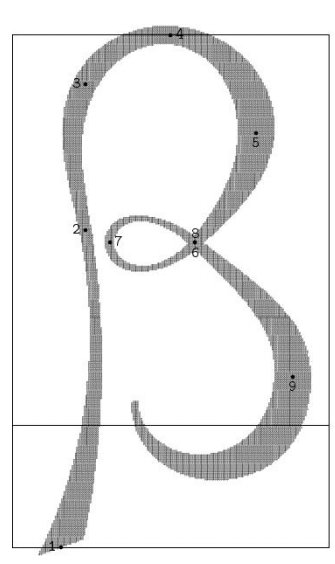
\includegraphics[scale=0.20]{beta}
\caption{Render of above MetaFont program}
\label{fig:fontrender}
\end{figure}

%% \begin{figure}
%% \begin{eqnarray*}
%%   \mbox{Program } p & := & \tt{Concat}(e_1, e_2, e_3, ...) \nonumber \\
%%   \mbox{Expression } e & := & f \; | \; n \; | \; n_1(n_2) \; | \; n(f) \; | \; \tt{ConstStr}(c) \nonumber \\
%%   \mbox{Substring } f & := & \tt{SubStr}(k_1,k_2)\\
%%   & | & \tt{GetSpan}(r_1,i_1,y_1,r_2,i_2,y_2) \nonumber \\
%%   \mbox{Nesting } \tt{n} & := & \tt{GetToken}(t, i) \; | \; \tt{ToCase}(s) \\
%%   & | & \tt{Replace}(\delta_1,\delta_2) \; | \; \tt{Trim}() \nonumber \\
%%   & | & \tt{GetUpto}(r) \; | \; \tt{GetFrom}(r) \\
%%   & | & \tt{GetFirst}(t,i) \; | \; \tt{GetAll}(t) \\
%%   \mbox{Regex } r & := & t_1 \; | \; \cdots \; | \; t_n \; | \; \delta_1 \; | \; \cdots \; | \; \delta_m \nonumber \\
%%   \mbox{Type } t & := & \tt{Number} \; | \; \tt{Word} \; | \; \tt{Alphanum} \nonumber \\
%%   & | & \tt{AllCaps} \; | \; \tt{PropCase} \; | \; \tt{Lower} \nonumber \\
%%   & | & \tt{Digit} \; | \; \tt{Char} \nonumber \\
%%   \mbox{Case } s & := & \tt{Proper} \; | \; \tt{AllCaps} \; | \; \tt{Lower} \nonumber \\
%%   \mbox{Position } k & := & -100, -99, ..., 1, 2, ... , 100 \nonumber \\
%%   \mbox{Index } i & := & -5, -4, -3, -2, 1, 2, 3, 4, 5 \nonumber \\
%%   \mbox{Character } c & := & \tt{A-Z},\tt{a-z},\tt{0-9},\tt{!?,@...} \nonumber \\
%%   \mbox{Delimiter } \delta & := & \tt{\&,.?!@()[]\%\{\}/:;\$\#"'}\ \nonumber \\
%%   \mbox{Boundary } y & := & \tt{Start} \; | \; \tt{End} \nonumber
%%   \end{eqnarray*}
%% \caption{Possible grammar to use}
%% \end{figure}

The contribution of this work is to introduce a system to generate a set of fonts for letters
directly from image data. The work has no prior knowledge of what alphabet the letters belong
to and only assumes they are non-overlapping in the image.

\section{Background}

\section{ABC}

Many of these drawing simulators don't have a nice tractable
likelihood, or would benefit from learning a tractable comparison
operator. Use \emph{approximate Bayesian computation} (ABC) we assume
you can generate data from a likelihood function along with the prior
distribution, but might not be able to evaluate the density of the
likelihood. Now to do better than a rejection sampler we don't
directly compare our generated data to our observed data, but instead
use a discrepancy function. We then sample from our parameters from the
prior distribution, sample from our likelihood function, and if
our discrepancy function says the generated and observed data are
close enough we accept this sample.

Traditionally, the discrepancy function uses some euclidean distance
between domain-specific summary statistics. For our discrepancy
function, we explore using the convolution filters from a pretrained
variational autoencoder (VAE).

\section{Related Work}

%% This work builds on several pieces of work. \citet{eslami2016attend} have been able to detect
%% multiple MNIST characters from a single image. Most similar is the work of \citet{ellis2018learning} which
%% learns to draw images from a subset of the \LaTeX\, language. In contrast to that work, we explicitly seek
%% to identify objects in the image and use our font language to then describe them. Additionally, we avoid
%% the use of an external problem synthesis system. This allows us to have a system which more consistently
%% generates a font from a given image by removing a search process from the overall system.

This work is inspired by the Omniglot challenge \citet{lake2015human}
which uses a grammar to describe each character as composed of a
series of parts and subparts of a character with subparts coming from
a library of primitive character strokes. A sampler is used to how
these parts and subparts are combined together to then form the
character. I have no idea how inference is done for the BPL models
that understand them to be a MCMC sampler with a carefully-chosen
proposal distribution.

Another piece of related work is
SPIRAL\citet{ganin2018synthesizing,mellor2019unsupervised}. This work
defines the drawing task as an adversarial RL task where they jointly
learn a discriminator and a generator with a WGAN loss. The
discriminator is trained to distinguish images from the data distribution
and images rendered from the strokes generated. The strokes are generated
using a RL policy that chooses a set of strokes to make given how the
rendered image looks as it draws. The agent is then trained using A2C
which is a form of \textsc{Reinforce}.

We instead choose to describe all characters are a sequence of
B-splines only selecting where each spline starts and ends. Our work
most closely follows the \citet{ha2017neural,chen2017sketch} which uses a CNN to
encode each image into a feature representation which is then fed into an
autoregressive model such as a LSTM which outputs stroke data.

\section{Model}
 
\begin{figure}[htb!]
\centering
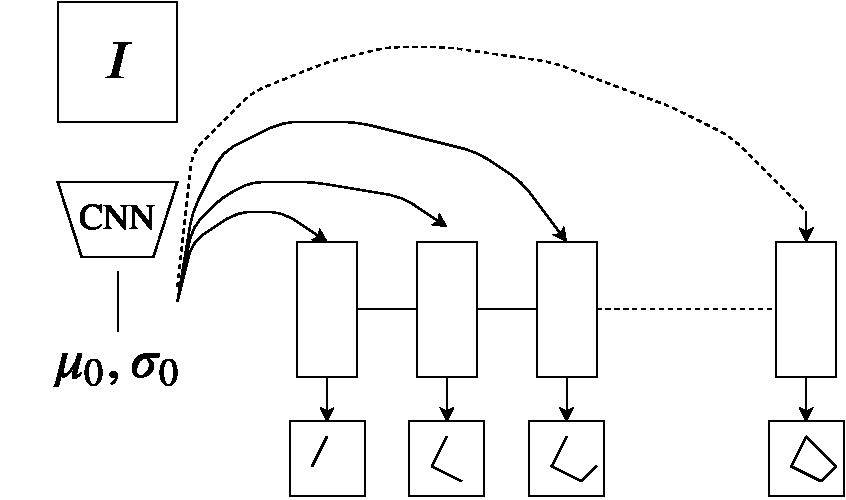
\includegraphics[scale=0.5]{omnisynthfig1.pdf}
\caption{Basic drawing model using a VAE model with a LSTM}
\label{fig:basicmodel}
\end{figure}


\begin{comment}
  2 and 3 are fine, Might add something about guide/proposal here as well if that makes sense.}
\end{comment}
    
We represent each stroke as B-spline. B-splines are piece-wise polynomials functions defined to be
continuous and differentiable. These strokes are defined in terms of the control points were these
piece-wise functions meet $t_1, t_2, \ldots, t_n$ called \emph{knots}. A B-spline with order-$n$
degree polynomials can then be defined recursively as follows.

\begin{equation}
B_{i,0}(x) := \left\{
\begin{matrix} 
1 & \mathrm{if} \quad t_i \leq x < t_{i+1} \\
0 & \mathrm{otherwise} 
\end{matrix}
\right.
\end{equation}

\begin{equation}
B_{i,k}(x) := \frac{x - t_i}{t_{i+k} - t_i} B_{i,k-1}(x) + \frac{t_{i+k+1} - x}{t_{i+k+1} - t_{i+1}} B_{i+1,k-1}(x).
\end{equation}

Our model extends the work of \citet{chen2017sketch} where we use a
variational autoencoder (VAE). Where a convolutional neural network
(CNN) $q_\phi($ is used to encode an image to some feature
representation. This feature representation is then fed into a RNN
$p_\theta(x \given y)$ which outputs control points $(s_x, s_y)$ for
each part of the spline $s_i$ along with signals for when to start and
end each spline.

\begin{eqnarray}
  p_\theta(s \given z) &=& \prod p_\theta(s_i \given s_{i-1}, z) \\
  p_\theta(s_i \given s_{i-1}, z) &=& \Gauss((\mu_x, \mu_y) , \Sigma) \\
  \mu_x, \mu_y, \Sigma &=& \text{LSTM}(s_{i-1}, z)
\end{eqnarray}

This stroke data is then rendered into an image. Our loss function can
then become $\E_{q_\phi(z \given z)}[\log p_\theta(x \given z)]$

While this, model is adequate for learning to draw an image. It's not
so good at capturing what makes something a particular letter. We will
try to capture the image in a series of glimpses that we try to
capture in a single stroke.  The style of strokes we settle on will
then give us a posterior on styles for an alphabet. We use a Spatial
Transformer Network\citep{jaderberg2015spatial} to decide on what
portion of the image to concentrate on, and then find a B-Spline to
draw it.

All the glimpses are then combined and compared with a pixel loss
to the original image.


\begin{figure}[htb!]
\centering
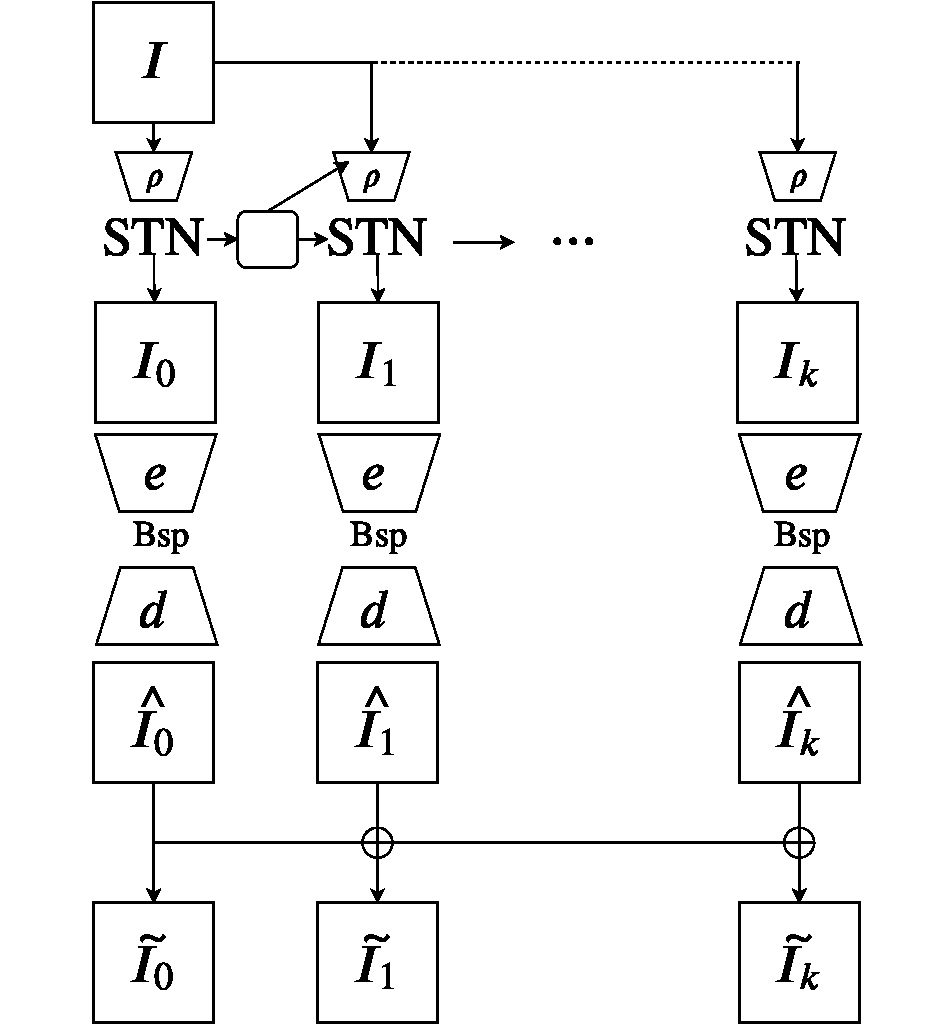
\includegraphics[scale=0.35]{omnisynthfig2.pdf}
\caption{Fancy drawing model using an AIR-like model with multiple glimpses for each stroke}
\label{fig:fancymodel}
\end{figure}

\begin{eqnarray}
  p(x, s) &=& \prod_{i=0}^K p(x_i \given \mu_i, \sigma_i)p(s_i^0 \cdots s_i^l)p(x \given \tilde{\mu_i},\tilde{\sigma_i}) \\
  q(s \given x) &=& \prod_{i=0}^K q(s \given x_i) \\
                &=& \prod_{i=0}^K q(s_i^0 \cdots s_i^l \given x_i)
\end{eqnarray}

\section{Learning}

\begin{comment}
  4 needs at least an outline of how you're planning on tacking things for learning..
Basically, we're going to be doing amortised VI which will let us learn the effective stroke set... tie this back to the motivation}
\end{comment}
  
We train our models in both a supervised manner and a completely
unsupervised manner. In a supervised manner, we use datasets of images
paired with their stroke data. In an unsupervised manner, we use a
VAE model we use only Omniglot images.


\section{Experiments}

\begin{figure}[htb!]
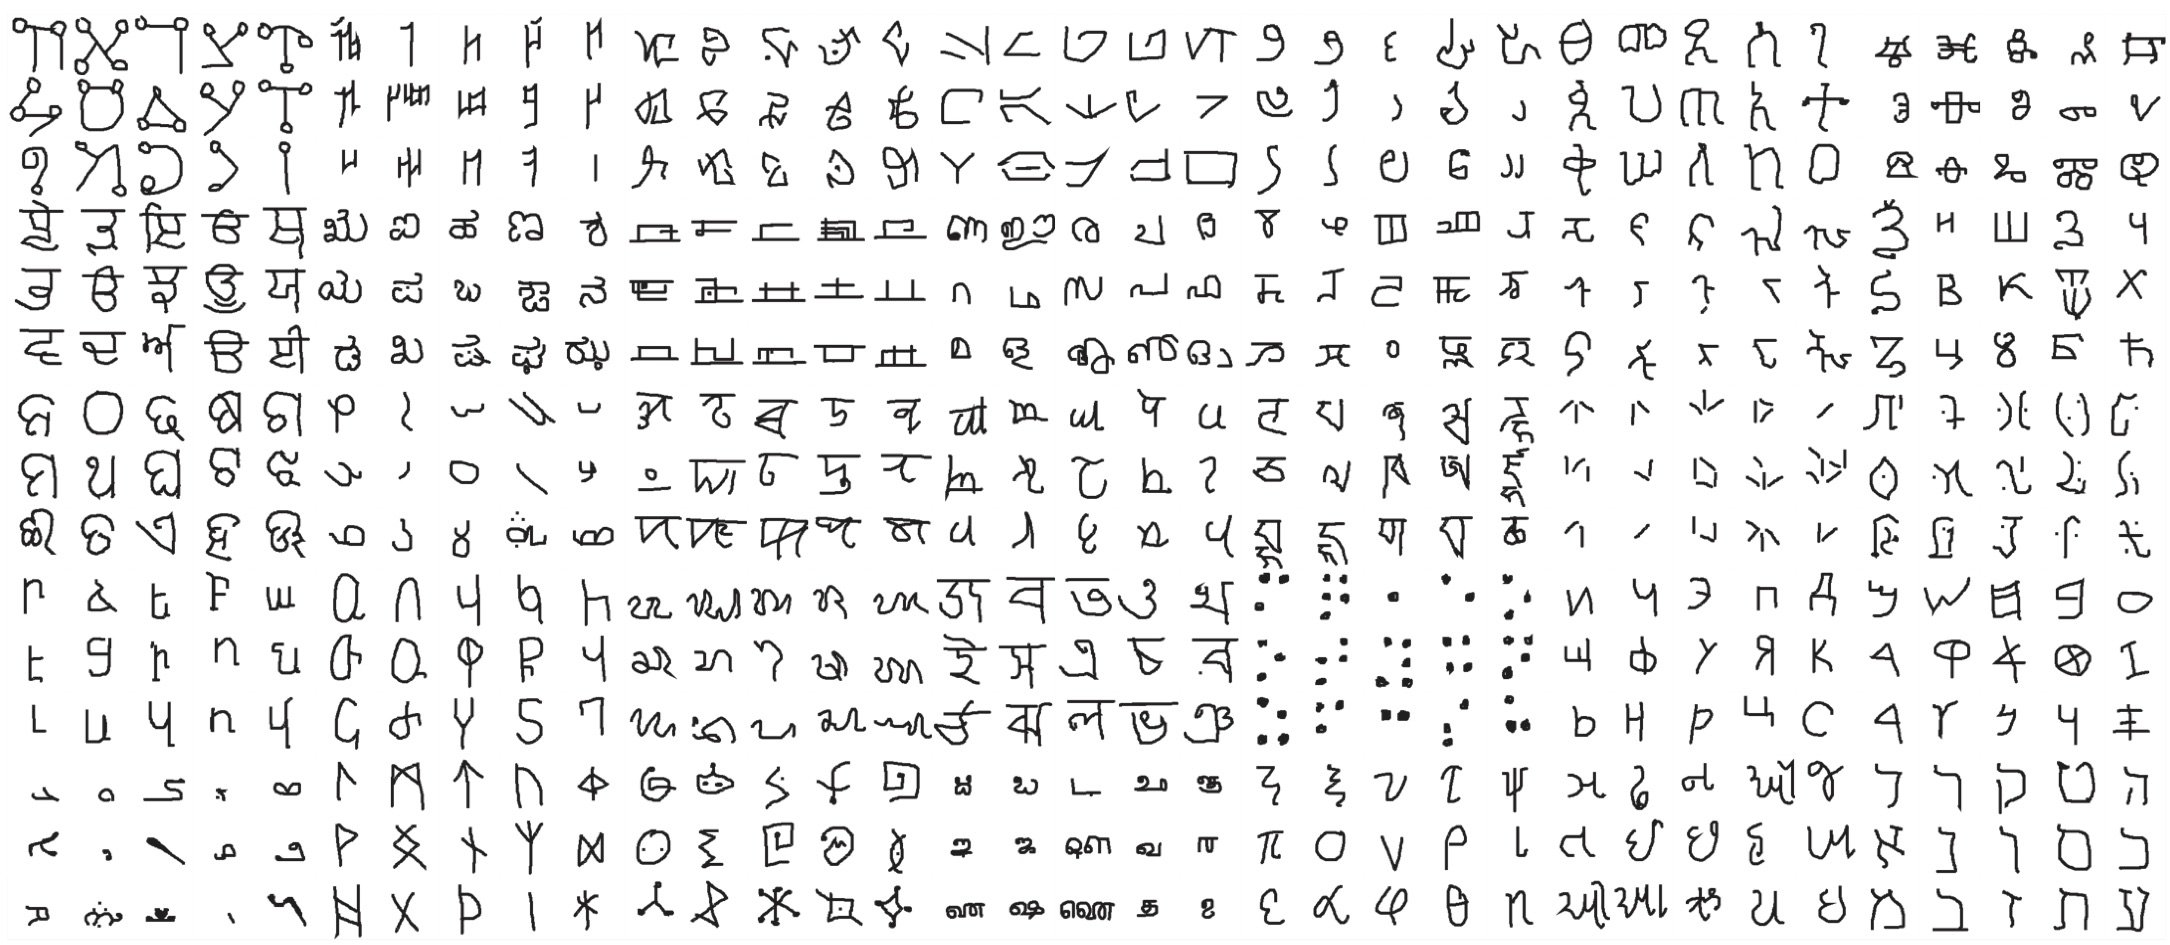
\includegraphics[scale=0.15]{omniglot_grid}
\caption{Omniglot characters}
\label{fig:omnigrid}
\end{figure}

A preliminary experiment was done with MNIST digits where we train a
VAE that has two convolutional layers emitting 10 and 20 channels with
a kernel size of 5 each. This is followed by two linear layers outputting
50 and then 90 units. These values and then used as control points for
a differentiable Bezier curve renderer.

We use a L1 pixel loss between the rendered image and the true
image. That is normalised by the L1 pixel distance between the
rendered image and an empty image. This is normalisation is to
encourage the control points to be within in the image boundaries.

Additionally, to have a less sparse gradient we use a Gaussian blurred
version of the rendered and true image for all our L1 pixel loss
comparisons. A neighbourhood of 7 pixels is used for the blur.

\begin{figure}[htb!]
\centering
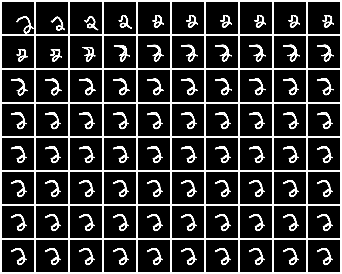
\includegraphics[scale=0.75]{../results/recons_gauss5}
\caption{Learning strokes from transposed letter using Adam}
\label{fig:shiftedinit}
\end{figure}

Another preliminary experiment involved using Hamiltonian Monte Carlo
(HMC) to learn to draw the character. This model uses a Beta(1, 1)
distribution for the control points with a Laplace distribution for
the likelihood distribution.

\begin{figure}[htb!]
\centering
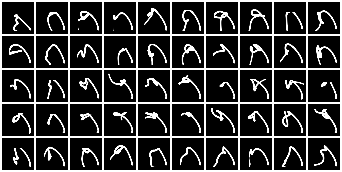
\includegraphics[scale=0.75]{../results/recons_pyro}
\caption{Learning strokes from transposed letter using HMC}
\label{fig:shiftedinithmc}
\end{figure}

Without normalisation training is not stable. This can be seen in
the following example where the same initialisation is used but
the loss function does not include normalisation against an empty
image or gaussian blurring.

\begin{figure}[htb!]
\centering
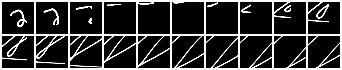
\includegraphics[scale=0.75]{../results/recons_nogauss}
\caption{Learning strokes from transposed letter}
\label{fig:shiftedinitnogauss}
\end{figure}

Further we explored if we can learn how to draw a character from
random initialisation. Training is still very sensitive to
initialisation. The following figures show training from 9 random
initialisation for a model with 5, 10, and 20 control points. The
character was generated from 20 control points.

\begin{figure}[htb!]
\centering
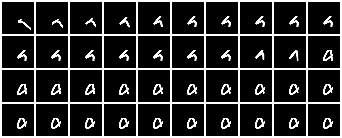
\includegraphics[scale=0.25]{../results/debug_recon/rand_init1.png}
%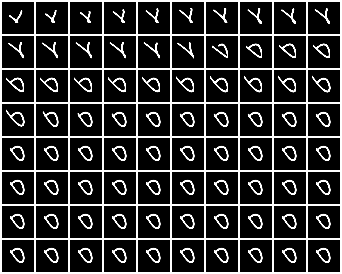
\includegraphics[scale=0.25]{../results/debug_recon/rand_init2.png}
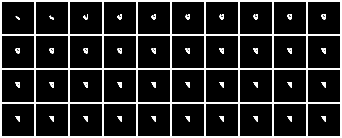
\includegraphics[scale=0.25]{../results/debug_recon/rand_init3.png}
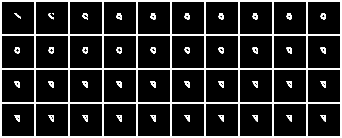
\includegraphics[scale=0.25]{../results/debug_recon/rand_init4.png}
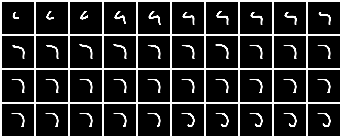
\includegraphics[scale=0.25]{../results/debug_recon/rand_init5.png}
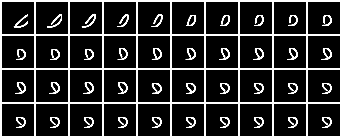
\includegraphics[scale=0.25]{../results/debug_recon/rand_init6.png}
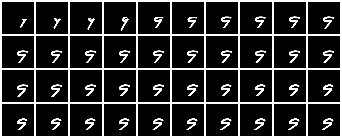
\includegraphics[scale=0.25]{../results/debug_recon/rand_init7.png}
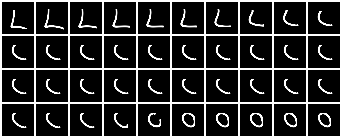
\includegraphics[scale=0.25]{../results/debug_recon/rand_init8.png}
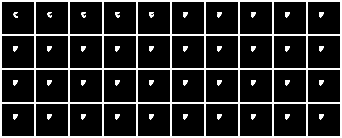
\includegraphics[scale=0.25]{../results/debug_recon/rand_init9.png}
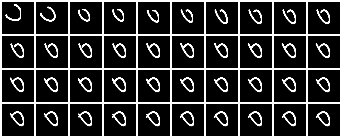
\includegraphics[scale=0.25]{../results/debug_recon/rand_init10.png}
\caption{Learning strokes from random initialisation with 5 control points}
\label{fig:shiftedinitrand5}
\end{figure}

\begin{figure}[htb!]
\centering
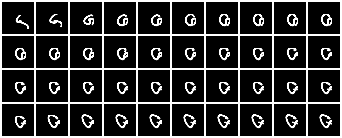
\includegraphics[scale=0.25]{../results/debug_recon/rand_init1_10.png}
%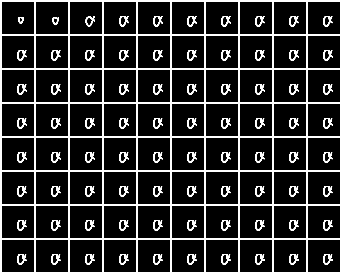
\includegraphics[scale=0.25]{../results/debug_recon/rand_init2_10.png}
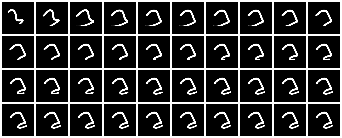
\includegraphics[scale=0.25]{../results/debug_recon/rand_init3_10.png}
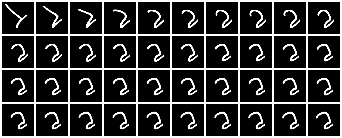
\includegraphics[scale=0.25]{../results/debug_recon/rand_init4_10.png}
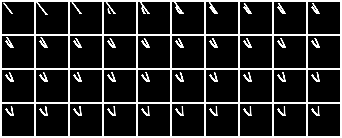
\includegraphics[scale=0.25]{../results/debug_recon/rand_init5_10.png}
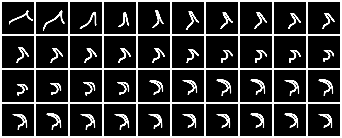
\includegraphics[scale=0.25]{../results/debug_recon/rand_init6_10.png}
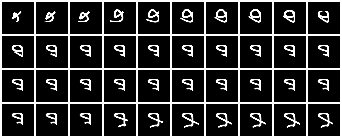
\includegraphics[scale=0.25]{../results/debug_recon/rand_init7_10.png}
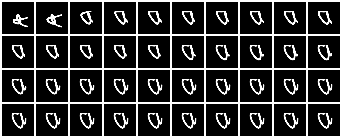
\includegraphics[scale=0.25]{../results/debug_recon/rand_init8_10.png}
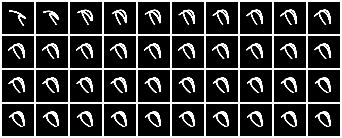
\includegraphics[scale=0.25]{../results/debug_recon/rand_init9_10.png}
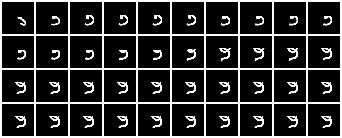
\includegraphics[scale=0.25]{../results/debug_recon/rand_init10_10.png}
\caption{Learning strokes from random initialisation with 10 control points}
\label{fig:shiftedinitrand10}
\end{figure}

\begin{figure}[htb!]
\centering
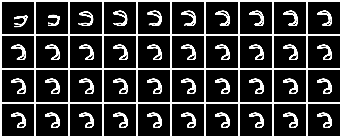
\includegraphics[scale=0.25]{../results/debug_recon/rand_init1_20.png}
%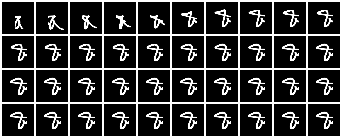
\includegraphics[scale=0.25]{../results/debug_recon/rand_init2_20.png}
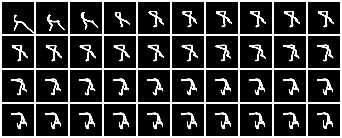
\includegraphics[scale=0.25]{../results/debug_recon/rand_init3_20.png}
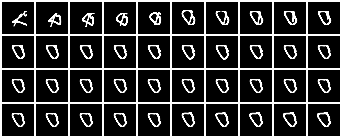
\includegraphics[scale=0.25]{../results/debug_recon/rand_init4_20.png}
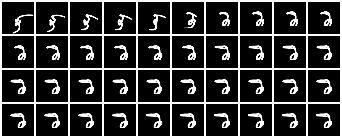
\includegraphics[scale=0.25]{../results/debug_recon/rand_init5_20.png}
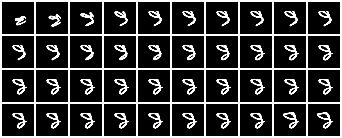
\includegraphics[scale=0.25]{../results/debug_recon/rand_init6_20.png}
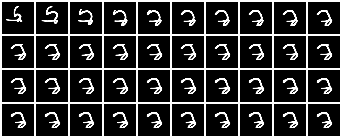
\includegraphics[scale=0.25]{../results/debug_recon/rand_init7_20.png}
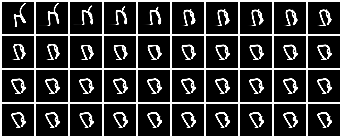
\includegraphics[scale=0.25]{../results/debug_recon/rand_init8_20.png}
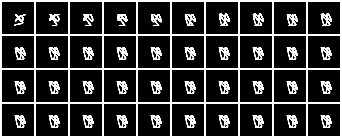
\includegraphics[scale=0.25]{../results/debug_recon/rand_init9_20.png}
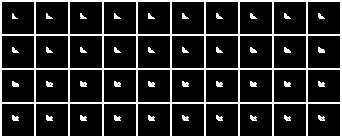
\includegraphics[scale=0.25]{../results/debug_recon/rand_init10_20.png}
\caption{Learning strokes from random initialisation with 20 control points}
\label{fig:shiftedinitrand20}
\end{figure}


Another initial experiment will learn to draw single letters from the Omniglot\citet{lake2015human} dataset.

%% This will be followed by a model that can identify and extract several
%% non-overlapping letters from an image.

This will be followed by experiments using EMNIST\citep{cohen1702emnist} and
KMNIST\citep{clanuwat2018deep}. The goal being to see if we can draw unseen letters of each
alphabet. This shows that we have a high degree of generalisation.

%% Omniglot challenge consists of
%% \begin{enumerate}
%% \item One-shot classification
%% \item Parsing
%% \item Generating new examples
%% \item Generating new concepts from type
%% \item Generating new concepts without type
%% \end{enumerate}


%% For learning layouts consider using STNs or outputting bounding boxes.

%% Variational RNN

%% Use a per glimpse loss, which are then put into a linear function


\bibliography{paper}
\bibliographystyle{unsrtnat}

\end{document}

%%  LocalWords:  convolutional autoregressive
